\documentclass{article}
\usepackage{amsmath}
\usepackage{amssymb}
\usepackage{listings}
\usepackage{xcolor}
\usepackage{graphicx}

\definecolor{codegreen}{rgb}{0,0.6,0}
\definecolor{codegray}{rgb}{0.5,0.5,0.5}
\definecolor{codepurple}{rgb}{0.58,0,0.82}
\definecolor{backcolour}{rgb}{0.95,0.95,0.92}

\lstdefinestyle{mystyle}{
    %backgroundcolor=\color{backcolour},   
    commentstyle=\color{codegreen},
    keywordstyle=\color{magenta},
    numberstyle=\tiny\color{codegray},
    stringstyle=\color{codepurple},
    basicstyle=\ttfamily\footnotesize,
    breakatwhitespace=false,         
    breaklines=true,                 
    captionpos=b,                    
    keepspaces=true,                 
    numbers=left,                    
    numbersep=5pt,                  
    showspaces=false,                
    showstringspaces=false,
    showtabs=false,                  
    tabsize=2,
}

\lstset{style=mystyle}


\title{Previous Exam solution}
\author{Michel Hardenberg}
\date{\today}
\begin{document}
\maketitle

\section*{Problem 1}
\subsection*{Periodicity}
\begin{description}
    \item[i)] $x(t) = 3\cos(3t + \pi/3)$ is periodic as it is a simple sinusoid with $T=\frac{2\pi}{3}$.
    \item[ii)] $x(t) = 3\cos^2(3t + \pi/3)$ is also periodic. To see this note that $y(t) = 3\cos(3t + \pi/3)$ is periodic as before. Then that $y(t + \frac{\pi}{3}) = -y(t)$. but since we take the square $x(t) = y^2(t) = y^2(t + \frac{\pi}{3})$ it now is periodic with half the period of $y(t)$, namely $T=\frac{\pi}{3}$.
\item[iii)] $x(t) = \cos(\frac{\pi}{2}t) + \cos(\frac{1}{2}t)$ is a sum of sinusoids with periods of $T_1 = 4$ and $T_2 = 4\pi$. $x(t)$ is periodic if there exist two integers $n,m$ such that $n\cdot T_1 = m\cdot T_2$. This is not possible as the fraction of $n/m \propto \pi$, which is irrational. Hence, no such integer numbers exist.

\item[iv)] $x(t) = e^{j\pi t}$ is trivially periodic, as it is a simple complex exponential and thus by Eulers rule, a sum of sinusoids of equal periods.
\end{description}

\subsection*{System properties}
\begin{equation}
    y(t) = x(t)x(t+2).
\end{equation}
\begin{description}
    \item[memoryless?] No, as the system depends on future values.
    \item[causal?] No, as the system depends on future values.
    \item[stable?] Yes. Let $x(t)$ be bounded by $|x(t)| < M < \infty$. Then 
    $|y(t)| = |x(t) \cdot x(t+2)| \leq M^2 < \infty$. Hence, $y(t)$ is bounded
    by $M^2$ for $M$ bounded input and thus stable.
    \item[TI] Yes. To be time invarient we need 
    \begin{equation}
        y(t + t_0) = x(t+t_0)x(t+2+t_0),
    \end{equation}
    which can be seen by insertion.

    \item[linear] No. Let $x(t) = a\cdot x_0(t) + b\cdot x_1(t)$. Then 

    \begin{align}
        x(t)x(t+2) &= (a\cdot x_0(t) + b\cdot x_1(t))
        (a\cdot x_0(t+2) + b\cdot x_1(t+2))\\
            &= a^2\cdot x_0(t)x_0(t+2) + b^2\cdot x_1(t)x_1(t+2) \nonumber\\
        &+ ab\cdot (x_0(t)x_1(t+2) + x_0(t+2)x_1(t))\\ 
            &\neq a\underbrace{\cdot x_0(t)x_0(t+2)}_{y(t)\mid _{x(t)=x_0(t)}}
        + b\cdot \underbrace{x_1(t)x_1(t+2)}_{y(t)\mid_{x(t) = x_1(t)}}.
    \end{align}
\end{description}

\begin{equation}
    y[n] = max\{x[n], x[n+1]\}.
\end{equation}

\begin{description}
    \item[memoryless?] No, as the system depends on future values.
    \item[causal?] No, as the system depends on future values.
    \item[stable?] Yes. Let $x(t)$ be bounded by $M$ as before. Then by definition 
    $y(t)$ is also bounded by $M$ and thus it is stable.
    \item[TI?] Yes. Any values we input will shift the output by the same. As 
    we compare to the one-setp-ahead value, we will always cover the same pairings. Different integer jumps could produce different pairing depending on time 
    delays of the imput and could be time variant.
    \item[Linear] No. Generally\footnote{There are exceptions, but that's not
    the point.}
    \begin{align}
        &a\cdot max\{x_0[n], x_0[n+1]\} + b\cdot max\{x_1[n],
        x_1[n+1]\}\nonumber\\
        &\neq max\{ax_0[n] + bx_1[n], ax_0[n+1] + bx_1[n+1]\}
    \end{align}
Consider e.g.
\begin{align}
    x_0[n] &= [\dots, 1, 2, 1, 2, \cdots]\\
    x_1[n] &= [\dots, 1, -1, 1, -1, \cdots]\\ 
\Rightarrow x_0[n]+x_1[n] &= [\dots, 2, 1, 2, 1, \dots]\text{ and }\\
    a&=b=1.
\end{align}

Then 
\begin{align}
    y_0[n] &= [\dots, 2, 2, 2, \dots]\\
    y_1[n] &= [\dots, 1, 1, 1, \dots]\\
\Rightarrow y_0[n]+y_1[n] &= [\dots, 3, 3, 3, \dots],
\end{align}

but
\begin{align}
    y_{x_0 + x_1}[n] &= [\dots, 2, 2, 2, \dots]\\
    &\neq y_0[n]+y_1[n].
\end{align}
\end{description}


\newpage

\section*{Problem 2 - Fourier series}
This exercise would usually require integration by parts, which we havn't used 
thorughout the course and will not appear in the final exam. I have sligtly 
changed the signal to make this problem more representative of the coming exam.
Let 
\begin{align}
    x(t) = \begin{cases}
        -2, &\text{ if }0\leq t < 1\\
        1, &\text{ if }1\leq t < 2\\
        0, &\text{ if }2\leq t < 4\\        
    \end{cases}
\end{align}

and $T = 4$. We know 
\begin{align}
    a_k &= \frac{1}{T}\int_T dt \ \ x(t)e^{-jk\frac{2\pi}{T}t}
        &= \frac{1}{4} (\int_0^1 dt \ \ -2 e^{-jk\frac{2\pi}{T}t} 
            + \int_1^2 dt \ \ e^{-jk\frac{2\pi}{T}t})
\end{align}

\newpage

\section*{Problem 3 LTI}
\subsection*{Frequency response}
Let $\dot{y}(t) + 3y(t) = x(t)$ be some LTI system.

We can solve the difference equation by using the Fourier transform.
\begin{align}
    \dot{y}(t) + 3y(t) &= x(t)\\
\Rightarrow j\omega Y(j\omega) + 3Y(j\omega) &= X(j\omega).
\end{align}

We now have eliminated the differential and can simply rearange as such
\begin{align}
   Y(j\omega)(j\omega  + 3) &= X(j\omega)\\ 
\Rightarrow \frac{Y(j\omega)}{X(j\omega)} &\equiv H(j\omega) = \frac{1}{j\omega + 3}
\end{align}

\subsection*{Bode plot}
You could just compute a few values and then sketch it by hand. Otherwise, here
is some code that does it.

\begin{lstlisting}[language=python]
# imports
import numpy as np
import matplotlib.pyplot as plt


# frequencies
ws = np.linspace(0, np.pi, 100)

# analytical frequency response
def f_rsp(w):
    return 1 / (1j * w + 3)
    
# convert to dB
def dB(s):
    return 20*np.log10(s)

# plot
fig, ax = plt.subplots()
ax.plot(ws, np.abs(f_rsp(ws)))
ax.set_title("Bode plot")
ax.set_xlabel(r"$\omega$")

plt.savefig("figures/p3_bode.png")
plt.show()
\end{lstlisting}

\begin{figure}[h!]
    \begin{center}
        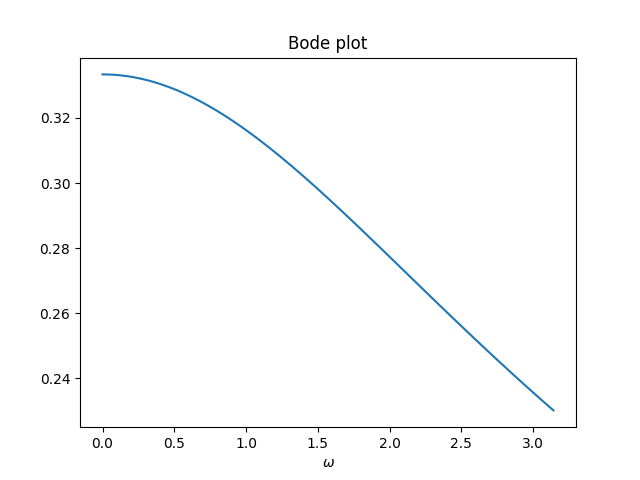
\includegraphics[width=0.75\textwidth]{figures/p3_bode.png}
    \end{center}
    \caption{Bode plot of system.}
\end{figure}


\newpage

\section*{Problem 4 LTI convolution}
Let 
\begin{align}
    h[n] = 2(u[n] - u[n-5]),
\end{align}

be an impulse response of some system and 
\begin{align}
    x[n] = u[n] - u[n-3]
\end{align}

the input.
\subsection*{Discrete case}
\subsubsection*{Scetch both}
\begin{lstlisting}[language=python]
# imports
import numpy as np
import matplotlib.pyplot as plt


# define series
def h_fn(n):
    return 2*(np.heaviside(n, 1) - np.heaviside(n-5, 1))

def x_fn(n):
    return np.heaviside(n, 1) - np.heaviside(n-3, 1)

# define ns
ns = np.arange(-3,10)


#plot 
fig, ax = plt.subplots()
ax.stem(ns, h_fn(ns), linefmt='tab:blue', label='h[n]')
ax.stem(ns, x_fn(ns), linefmt='tab:orange', label='x{n]')

ax.legend()
plt.savefig("figures/p4_stems.png")
plt.show()
\end{lstlisting}
\clearpage

\begin{figure}[h!]
    \begin{center}
        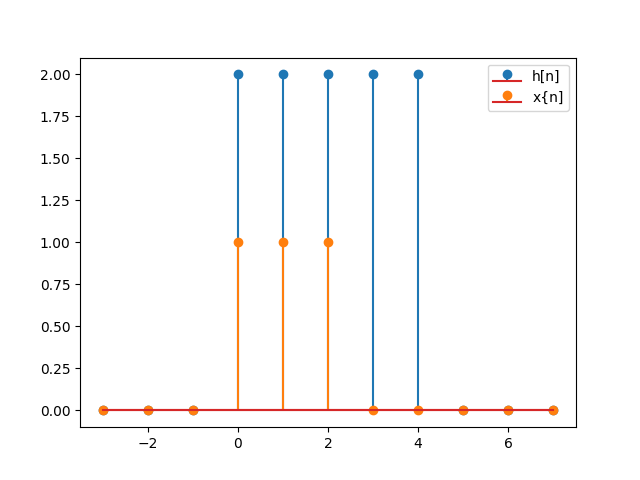
\includegraphics[width=0.95\textwidth]{figures/p4_stems.png}
    \end{center}
    \caption{Input and impulse response.}
\end{figure}

\subsubsection*{Sketch the convolution}
\begin{lstlisting}[language=python]
ys = np.convolve(xs, hs)
ks = np.arange(-(n + n), m + m - 1)

#plot 
fig, ax = plt.subplots()
ax.stem(ks, ys, linefmt='tab:green', label='y[n]')
ax.set_xlim([-3, 10])
ax.legend()
plt.savefig("figures/p4_conv.png")
plt.show()
\end{lstlisting}
\clearpage

\begin{figure}[h!]
    \begin{center}
        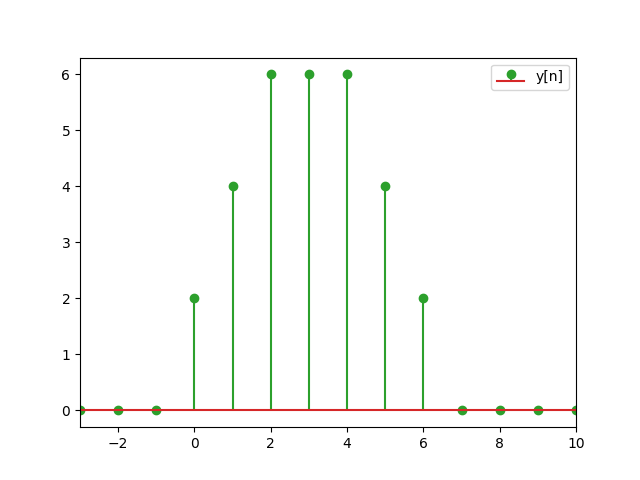
\includegraphics[width=0.95\textwidth]{figures/p4_conv.png}
    \end{center}
    \caption{Output.}
\end{figure}

\subsection*{Continuous case}
Let 
\begin{align}
    h(t) = (u(t) - u(t)),
\end{align}

be an impulse response of some system and 
\begin{align}
    x(t) = u(t) - u(t-3)
\end{align}

the input.
\subsubsection*{Scetch both}
\begin{lstlisting}[language=python]
# imports
import numpy as np
import matplotlib.pyplot as plt


# define series
def h_fn(t):
    return np.heaviside(t, 1) - np.heaviside(t-5, 1)

def x_fn(t):
    return np.heaviside(t, 1) - np.heaviside(t-3, 1)

# define ns
n, m = 3, 8
ts = np.linspace(-n, m, 100)
xs, hs = x_fn(ts), h_fn(ts)

#plot 
fig, ax = plt.subplots()
ax.plot(ts, hs, label='h[n]')
ax.plot(ts, xs, label='x{n]')

ax.legend()
plt.savefig("figures/p4_stems_ct.png")
plt.show()
\end{lstlisting}
\clearpage

\begin{figure}[h!]
    \begin{center}
        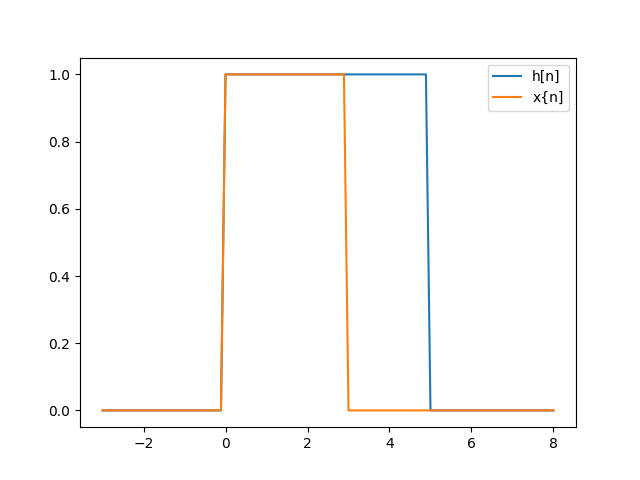
\includegraphics[width=0.95\textwidth]{figures/p4_stems_ct.png}
    \end{center}
    \caption{Input and impulse response.}
\end{figure}

\subsection*{Sketch convolution}
We find this by integration
\begin{align}
    y(t)    &= h(t)*x(t)\\ 
            &= \int_\mathbb{R}d\lambda \ \ h(\lambda)x(t-\lambda)\\
            &= \int_\mathbb{R}d\lambda \ \ (u(\lambda) - u(\lambda-5))
                (u(t-\lambda) - u(t-\lambda-3))\\
            &= \int_0^5d\lambda \ \ u(t-\lambda) - u(t-\lambda-3)\\ 
            &= \int_0^5 d\lambda \ \ u(t-\lambda) 
                - \int_0^5 d\lambda \ \ u(t - \lambda - 3).
\end{align}

Then 
\begin{align}
    y(t) &= \begin{cases}
    0, &\text{ if }t<0\\
    \int_0^t d\lambda = t, &\text{ if }0\leq t<3\\
        \int_0^t d\lambda  - \int_0^{t-3} d\lambda 
            \ \ = 3, &\text{ if }3\leq t<5\\
        \int_0^5 d\lambda  - \int_0^{t -3} d\lambda \ \ 
            = 8 - t, &\text{ if }t\leq 8\\
    0, &\text{ if }t >8\\
\end{cases}
\end{align}


\begin{lstlisting}[language=python]
def ys_fn(t):
    out = np.zeros_like(t)
    out[t < 8] = 8. -t[t<8]
    out[t < 5] = 3.
    out[t < 3] = t[t<3]
    out[t<0] = 0.

    return out

ts = np.linspace(-(n + n), m + m - 1, 100)
ys = ys_fn(ts)

#plot 
fig, ax = plt.subplots()
ax.plot(ts, ys, 'tab:green', label='y[n]')
ax.set_xlim([-3, 10])
ax.legend()
plt.savefig("figures/p4_conv_ct.png")
plt.show()
\end{lstlisting}

\clearpage

\begin{figure}[h!]
    \begin{center}
        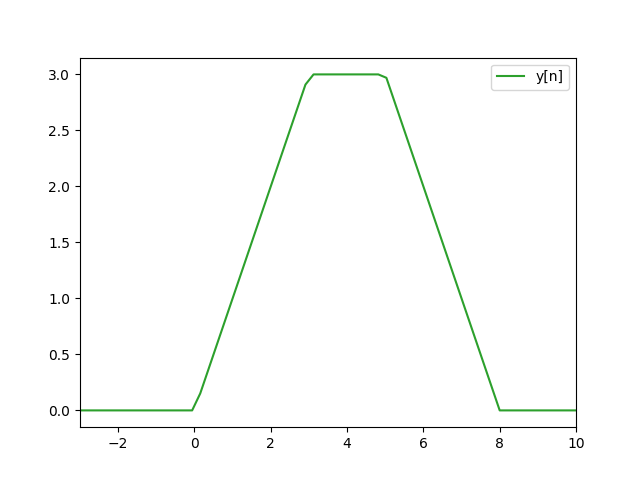
\includegraphics[width=0.95\textwidth]{figures/p4_conv_ct.png}
    \end{center}
    \caption{Output.}
\end{figure}

Unsurpirisngly this looks alot like the d.t. case.


\newpage

\section*{Problem 5 Laplace}
These types of question are part of the curriculum but not of the qualification
description or ”Kvalifikationsbeskrivelse” and will not be assessed in the
final exam.

\newpage
\end{document}
